% inspired from http://tex.stackexchange.com/questions/268128/how-to-nicely-place-two-heaps-next-to-each-other
\documentclass{article}

\usepackage{tikz}
\usepackage{array}
\usetikzlibrary{shapes.multipart}

\tikzset{
   heap/.style={
      every node/.style={circle, draw, fill=blue!20},
      level 1/.style={sibling distance=35mm},
      level 2/.style={sibling distance=20mm},
      level 3/.style={sibling distance=8mm}
   }
}

\begin{document}

% Exemple de tas max

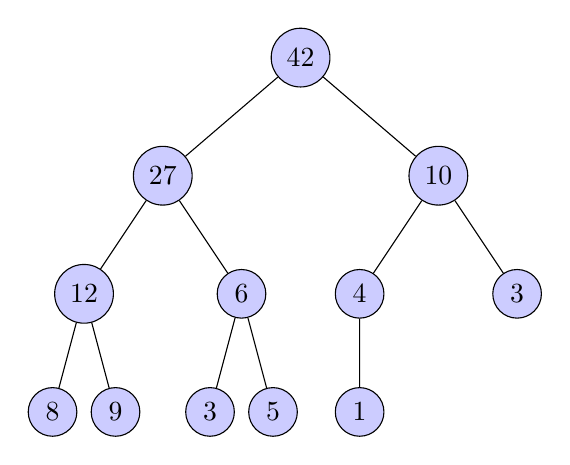
\begin{tikzpicture}[heap]
   \node {42}
   child{node{27}
      child{
         node{12}
         child{node{8}}
      child{node{9}}}
      child{node{6}
         child{node{3}}
   child{node{5}}}}
   child{node{10}
      child{node{4}
      child{node{1}}}
   child{node{3}}}
   ;
\end{tikzpicture}

\vspace{1cm}

% Tableau représentatif du tas

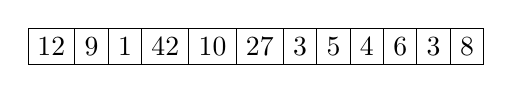
\begin{tikzpicture}
   \node[rectangle split, rectangle split horizontal, rectangle split parts = 12, draw]
   {
      \nodepart{one}12
      \nodepart{two}9
      \nodepart{three}1
      \nodepart{four}42
      \nodepart{five}10
      \nodepart{six}27
      \nodepart{seven}3
      \nodepart{eight}5
      \nodepart{nine}4
      \nodepart{ten}6
      \nodepart{eleven}3
      \nodepart{twelve}8
   };
\end{tikzpicture}

% Exemple insertion dans un tas max

\newpage

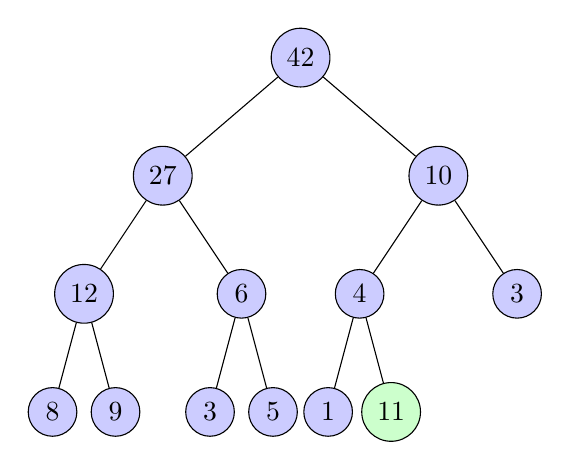
\begin{tikzpicture}[heap]
   \node {42}
   child{node{27}
      child{
         node{12}
         child{node{8}}
      child{node{9}}}
      child{node{6}
         child{node{3}}
   child{node{5}}}}
   child{node{10}
      child{node{4}
         child{node{1}}
      child{node[fill=green!20]{11}}}
   child{node{3}}}
   ;
\end{tikzpicture}
\hspace{1.5cm}
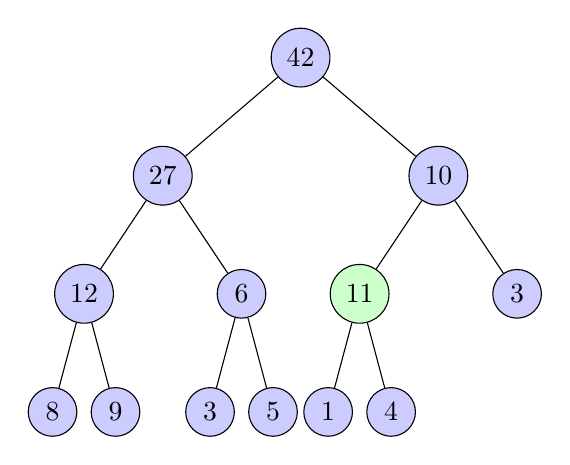
\begin{tikzpicture}[heap]
   \node {42}
   child{node{27}
      child{
         node{12}
         child{node{8}}
      child{node{9}}}
      child{node{6}
         child{node{3}}
   child{node{5}}}}
   child{node{10}
      child{node[fill=green!20]{11}
         child{node{1}}
      child{node{4}}}
   child{node{3}}}
   ;
\end{tikzpicture}

\vspace{1cm}
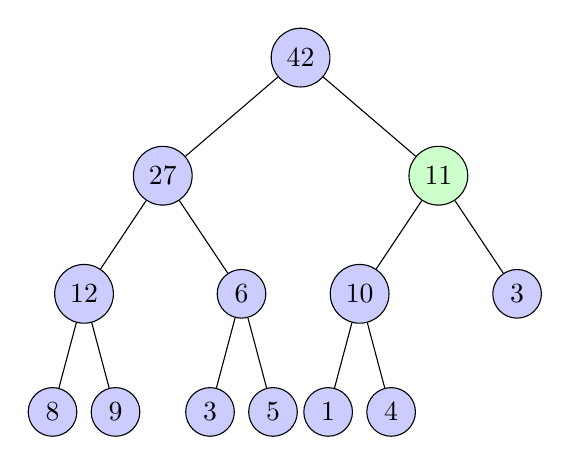
\begin{tikzpicture}[heap]
   \node {42}
   child{node{27}
      child{
         node{12}
         child{node{8}}
      child{node{9}}}
      child{node{6}
         child{node{3}}
   child{node{5}}}}
   child{node[fill=green!20]{11}
      child{node{10}
         child{node{1}}
      child{node{4}}}
   child{node{3}}}
   ;
\end{tikzpicture}

% Exemple extraction dans un tas max

\newpage

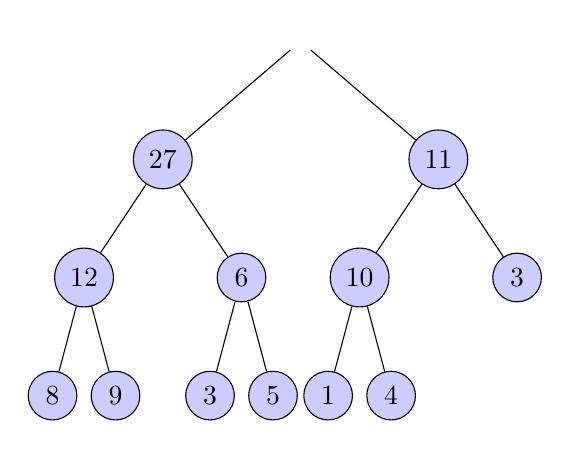
\begin{tikzpicture}[heap]
   \node[fill=white, draw=white]{}
   child{node{27}
      child{
         node{12}
         child{node{8}}
      child{node{9}}}
      child{node{6}
         child{node{3}}
   child{node{5}}}}
   child{node{11}
      child{node{10}
         child{node{1}}
      child{node{4}}}
   child{node{3}}}
   ;
\end{tikzpicture}
\hspace{1cm}
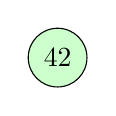
\begin{tikzpicture}
   \node[draw, circle, fill=green!20]{42};
\end{tikzpicture}

\vspace{1cm}
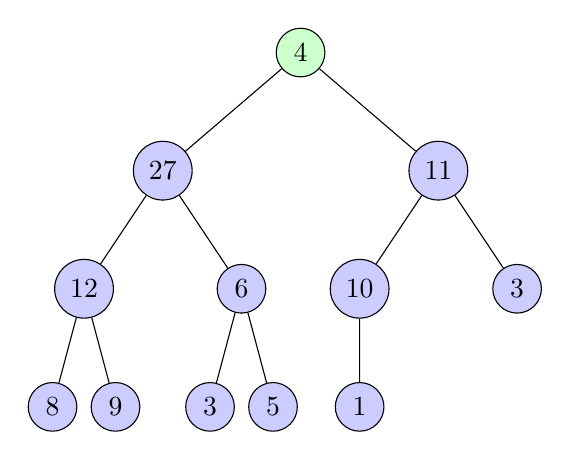
\begin{tikzpicture}[heap]
   \node[fill=green!20]{4}
   child{node{27}
      child{
         node{12}
         child{node{8}}
      child{node{9}}}
      child{node{6}
         child{node{3}}
   child{node{5}}}}
   child{node{11}
      child{node{10}
      child{node{1}}}
   child{node{3}}}
   ;
\end{tikzpicture}
\hspace{1.5cm}
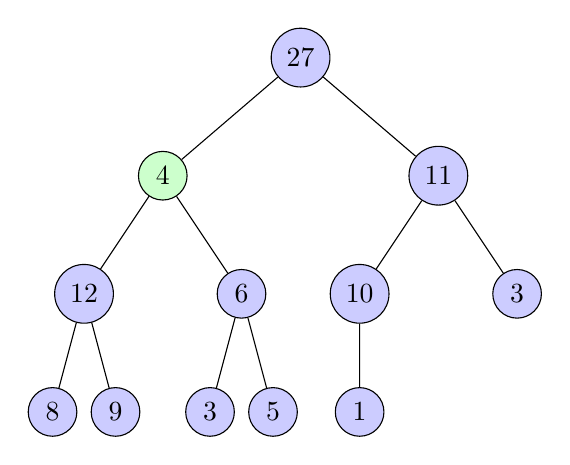
\begin{tikzpicture}[heap]
   \node{27}
   child{node[fill=green!20]{4}
      child{
         node{12}
         child{node{8}}
      child{node{9}}}
      child{node{6}
         child{node{3}}
   child{node{5}}}}
   child{node{11}
      child{node{10}
      child{node{1}}}
   child{node{3}}}
   ;
\end{tikzpicture}

\vspace{1cm}
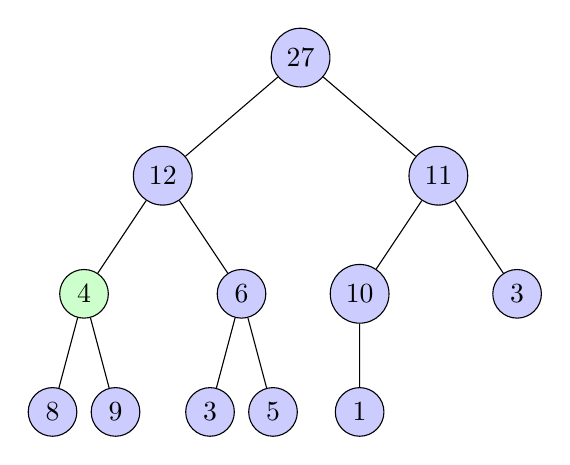
\begin{tikzpicture}[heap]
   \node{27}
   child{node{12}
      child{
         node[fill=green!20]{4}
         child{node{8}}
      child{node{9}}}
      child{node{6}
         child{node{3}}
   child{node{5}}}}
   child{node{11}
      child{node{10}
      child{node{1}}}
   child{node{3}}}
   ;
\end{tikzpicture}
\hspace{1.5cm}
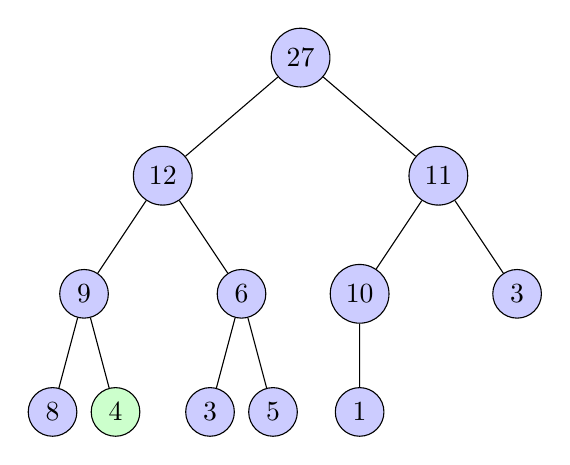
\begin{tikzpicture}[heap]
   \node{27}
   child{node{12}
      child{
         node{9}
         child{node{8}}
      child{node[fill=green!20]{4}}}
      child{node{6}
         child{node{3}}
   child{node{5}}}}
   child{node{11}
      child{node{10}
      child{node{1}}}
   child{node{3}}}
   ;
\end{tikzpicture}

\end{document}
